\documentclass[preview,border=2pt]{standalone}
\usepackage{times}
\usepackage{amsmath,amssymb}
\usepackage{siunitx}
\usepackage{tikz}
\usetikzlibrary{arrows.meta,positioning,fit,backgrounds,calc}
\DeclareTextFontCommand{\textsc}{\upshape\scshape}
\begin{document}
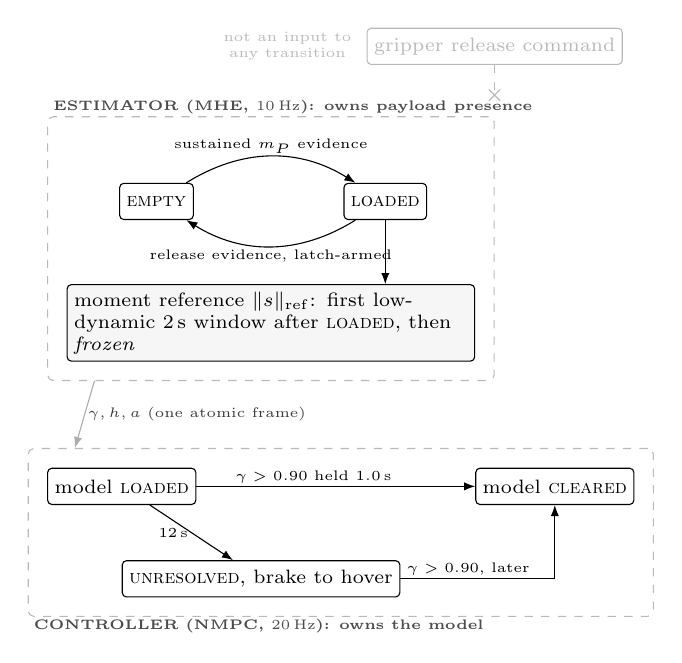
\begin{tikzpicture}[
  st/.style={draw,rounded corners=1.5pt,align=center,inner sep=2.5pt,
             minimum height=4.6mm,font=\scriptsize},
  ar/.style={-{Latex[length=1.4mm]},thin},
  lb/.style={font=\tiny,align=center,inner sep=1pt},
  lane/.style={draw=gray!55,dashed,rounded corners=2pt,inner sep=2.4mm},
  hd/.style={font=\tiny\bfseries,text=gray!60!black,inner sep=0.6pt},
]
% ============ estimator lane ============
\node[st] (empty) {\textsc{empty}};
\node[st,right=19mm of empty] (loaded) {\textsc{loaded}};
\draw[ar] (empty) to[out=32,in=148]
  node[lb,above,pos=.5] (lab1) {sustained $m_P$ evidence} (loaded);
\draw[ar] (loaded) to[out=212,in=-32]
  node[lb,below,pos=.5] (lab2) {release evidence, latch-armed} (empty);
\node[st,below=10.5mm of $(empty)!0.5!(loaded)$,fill=gray!7,text width=50mm,align=left]
  (ref) {moment reference $\lVert s\rVert_{\mathrm{ref}}$: first low-dynamic
         \SI{2}{s} window after \textsc{loaded}, then \emph{frozen}};
\draw[ar] (loaded.south) -- (loaded.south|-ref.north);
\begin{scope}[on background layer]
  \node[lane,fit=(empty)(loaded)(ref)(lab1)(lab2)] (elane) {};
\end{scope}
\node[hd,anchor=south west] at ([xshift=0.5mm]elane.north west)
  {ESTIMATOR (MHE, \SI{10}{Hz}): owns payload presence};
% ============ command, not consumed ============
\node[st,draw=gray!55,text=gray!55,anchor=south east,
      above=6.5mm of elane.north east] (cmd) {gripper release command};
\draw[gray!55,dashed,thin] (cmd.south) -- ++(0,-3.2mm);
\node[font=\scriptsize,text=gray!55,inner sep=0pt]
  at ([yshift=-3.9mm]cmd.south) {$\boldsymbol\times$};
\node[lb,text=gray!55,anchor=east] at ([xshift=-1.5mm]cmd.west)
  {not an input to\\any transition};
% ============ controller lane ============
\node[st,below=11mm of elane.south west,anchor=north west] (mload) {model \textsc{loaded}};
\node[st,below=7mm of mload,anchor=north west] (unres) {\textsc{unresolved}, brake to hover};
\node[st,anchor=west] at (mload-|ref.east) (clear) {model \textsc{cleared}};
\draw[ar] (mload) -- node[lb,above,pos=.42] (lab3) {$\gamma>0.90$ held \SI{1.0}{s}} (clear);
\draw[ar] (mload) -- node[lb,left,pos=.5] {\SI{12}{s}} (unres);
\draw[ar] (unres.east) -| node[lb,above,pos=.22] {$\gamma>0.90$, later} (clear.south);
\begin{scope}[on background layer]
  \node[lane,fit=(mload)(unres)(clear)(lab3)] (clane) {};
\end{scope}
\node[hd,anchor=north west] at ([xshift=0.5mm]clane.south west)
  {CONTROLLER (NMPC, \SI{20}{Hz}): owns the model};
\draw[ar,gray!65] ([xshift=6mm]elane.south west) -- ([xshift=6mm]clane.north west)
  node[lb,right,pos=.5,text=gray!45!black] {$\gamma,h,a$ (one atomic frame)};
\end{tikzpicture}
\end{document}
